%%
%% This is file `tikzposter-example.tex',
%% generated with the docstrip utility.
%%
%% The original source files were:
%%
%% tikzposter.dtx  (with options: `tikzposter-example.tex')
%% 
%% This is a generated file.
%% 
%% Copyright (C) 2014 by Pascal Richter, Elena Botoeva, Richard Barnard, and Dirk Surmann
%% 
%% This file may be distributed and/or modified under the
%% conditions of the LaTeX Project Public License, either
%% version 2.0 of this license or (at your option) any later
%% version. The latest version of this license is in:
%% 
%% http://www.latex-project.org/lppl.txt
%% 
%% and version 2.0 or later is part of all distributions of
%% LaTeX version 2013/12/01 or later.
%% 
 \documentclass[17pt, a1paper, portrait, margin=0mm, innermargin=1mm,
     blockverticalspace=3mm, colspace=5mm, subcolspace=5mm]{tikzposter} %Default values for poster format options.

\tikzposterlatexaffectionproofoff %shows small comment on how the poster was made at bottom of poster
\usepackage{exscale}
\usepackage{listings}
\usepackage[hidelinks]{hyperref}
\usepackage{wrapfig}
\usepackage[backend=biber, sorting=none]{biblatex}
\usepackage{framed}
\usetikzlibrary{backgrounds}
\pgfmathsetseed{1} % To have predictable results
% Define a background layer, in which the parchment shape is drawn

\addbibresource[datatype=bibtex]{dmposter.bib}
\geometry{paperwidth=24in, paperheight=36in}


 % Commands
 \newcommand{\bs}{\textbackslash}   % backslash
 \newcommand{\cmd}[1]{{\bf \color{red}#1}}   % highlights command
 \usepackage{float}
 \floatstyle{boxed}
 \restylefloat{figure}

 % Title, Author, Institute
\title{Can Twitter User's Moods Predict the Stock Market?}
\author{Aaron Gonzales and Adam Delora}
\institute{Department of Computer Science, University of New Mexico} 
%\titlegraphic{UNM_SOE_Logo_Color}

 % -- PREDEFINED THEMES ---------------------- %
 % Choose LAYOUT:  Default, Basic, Rays, Simple, Envelope, Wave, Board, Autumn, Desert,
\usetheme{Basic}
\usecolorstyle[colorPalette=BrownBlueOrange]{Germany}


 \begin{document}

 \maketitle[width=55cm, titletotopverticalspace=0.0cm]

 \begin{columns}%blocks will be placed into columns
   \column{.50}
%%%%%%%%%%%%%%%%new block%%%%%%%%%%%%%%%%%%%%%%%%%%%%%%%%%%%%
   \block{Background}{
     \begin{itemize}
       \item Twitter is a microblogging service with 284 million monthly
         active users who post 500 million updates (``tweets'') per day.
     \item Latent Semantic Indexing\cite{lsipaper} is a
       technique used to summarize words (documents) into representative ideas
       similar to principle component analysis.
       \item The AFINN semantic indexing database \cite{ANEW} assigns coded valence
         values to common words to allow quantification of a set of word's
         ``mood''.
     \end{itemize}
   }
%%%%%%%%%%%%%%%%new block%%%%%%%%%%%%%%%%%%%%%%%%%%%%%%%%%%%%
   \block{Methods}{
     We collected tweets using the public Twitter Streaming RESTful API
     over 2014-10-17 \textemdash 2014-11-09 by tracking words that related
     to various tech stocks indexed by NASDAQ. Tweets were stored in a Mongo
     noSQL database.
     \begin{tikzfigure}[Several examples of de-identified tweets from our
       dataset] 
       \label{fig:tweets}
       \begin{itemize}
         \item \small{Maine nurse defies Ebola quarantine order by taking bike ride.
           http://t.co/eERINkm3AQ via @indystarJ}
         \item \small{Tim Cook: Apple CEO Says 'Being Gay Is One Of God's
             Greatest Gifts' Earlier today, the chief executive of
             Apple,\ldots \url{http://t.co/zIXb2HbDmd}}
         \item \small{ Meet the Swedish twin sisters who want to be
             'identical artificial dolls' \url{http://t.co/77eA3esaQa}}
         \item \small{Last Christmas I got a black iPhone it was the
           worst Christmas present ever, I wanted a white one. I mean I'm
           not\ldots \url{http://t.co/jhP9ODs3QK}}
       \end{itemize}
         \tiny{\textcolor{white}{blah}}
     \end{tikzfigure}
    %\begin{wrapfigure}[6]{l}{0.33\linewidth}
     \begin{tikzfigure}[Kewords tracked] \label{fig:keywords}
       
\begin{tikzpicture}[background rectangle/.style={fill=black},show
         background rectangle]
         \node[anchor=north west] (note2) at (0,0)
         { \small{ebola, aapl, apple, mac, tim cook, goog,
           youtube, microsoft, msft }};
         \node[anchor=north west] (note2) at (0,0.5)
         { \small{nadella, twrt, amazon, amzn, prime, aws, fb,
         facebook, google, gmail,}};

       \end{tikzpicture}
     \end{tikzfigure}
    %\end{wrapfigure}
     NASDAQ market data was collected over a slightly longer period, 2014-08-30
     - 2014-11-09. Apple (aapl), Amazon (amzn), Facebook (fb), Google (goog),
     Microsoft (msft), and Twitter (twtr) stocks were analyzed using their
     hourly closing price. Tweet text was preprocessed to remove common
     stopwords and punctuation and each hour bin was represented as a
     bag-of-words vector. Latent semantic indexing was performed on the
     one-hour bins of tweets, giving a total of 218 hours included in analysis.
     Each hour's LSI topics were scored using the AFINN database, resulting in
     a single number indicating semantic valence for each hour.  The LSI score
     was smoothed using rolling means and assessed for periodicity. Semantic
     data was combined with the stock data and standardized for visualization
     (see Figure \ref{fig:means})
     and analysis. A model was created using vector autoregression (VAR) to
     assess 	the predictive power of the semantic data against the stock data.
     All work was done using Python: Tweets were harvested using
     Tweepy\cite{tweepy}, text preprocessing was performed using Gensim
     \cite{rehurek_lrec}, visualizations were made with
     Matplotlib\cite{Hunter:2007}, and statistical analysis was performed with
     Statsmodels \cite{statsmodels2010}. 

     Within an hour bin, LSI would provide a set of topics as noted in Figure
     \ref{tab:topics}. Representative Word clouds were generated for each hour
     as shown in Figure \ref{fig:wordcloud}.
     \begin{tikzfigure}[Two LSI topics from 2014-10-16, 14:00 - 15:00]
       \label{tab:topics}
       \begin{tabular}{|c|c|c|c|c|c|c|c|c|c|}
         \hline
         scientists & are   & about & do    & don't & over  & say   & climate & it    & panic \\ 
         \hline
         0.416      & 0.219 & 0.217 & 0.216 & 0.214 & 0.211 & 0.209 & 0.209   & 0.209 & 0.208 \\ 
         \hline
         %\end{tabular}
         %\begin{tabular}{|c|c|c|c|c|c|c|c|c|c|}
         \hline
         on    & is     & get    & from  & ebola  & i      & google & it     & really & liked \\ 
         \hline
         0.586 & -0.315 & -0.217 & 0.165 & -0.140 & -0.129 & -0.126 & -0.122 & -0.117 & 0.208 \\ 
         \hline
       \end{tabular}
     \end{tikzfigure}
   } 
%%%%%%%%%%%%%%%%new block%%%%%%%%%%%%%%%%%%%%%%%%%%%%%%%%%%%%
     \block{Summary, Descriptive Statistics}{
       \begin{itemize}
         \item \small{Total tweets collected: 84 million}
         \item \small{Total hours analyzed: 218}
         \item \small{Number of tweets per hour: 205,200; std 71,700}
         \item \small{Mean semantic score:  4.78; std 1.39}
       \end{itemize}
       %\begin{wrapfigure}{l}{0.8\linewidth}
       \begin{tikzfigure}[Word clouds generated from topics on 2014-10-30,
         11:00-12:00 and 12:00 - 13:00. The LSI model was able to capture
       information about Tim Cook (Apple's CEO) coming out as gay on that day.]
         \label{fig:wordcloud}
         {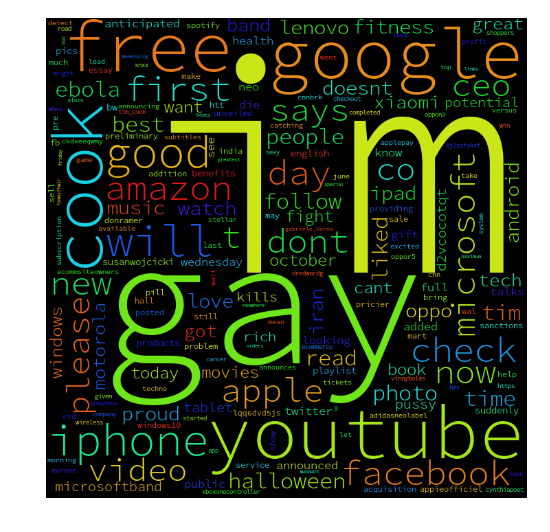
\includegraphics[width=0.49\linewidth]{../analysis/img170.png}}
         {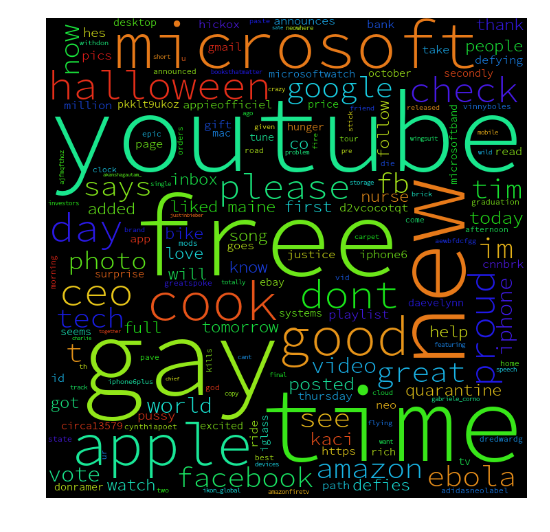
\includegraphics[width=0.49\linewidth]{../analysis/img173.png}}
         %{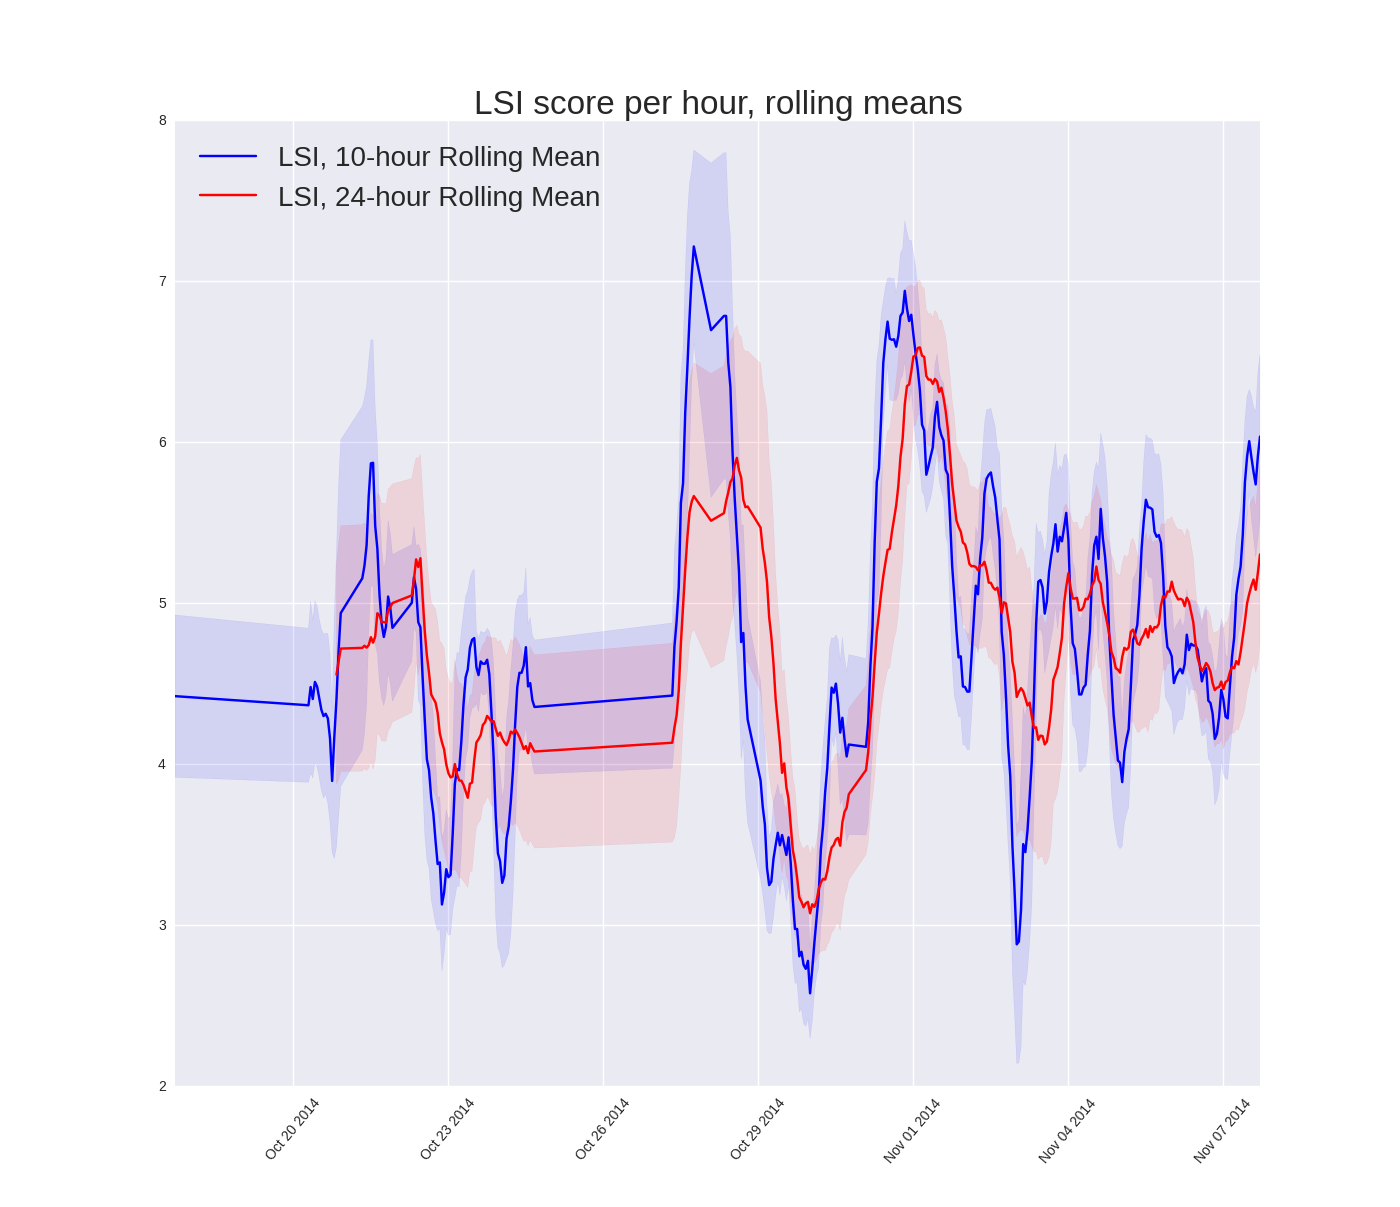
\includegraphics[width=0.46\linewidth]{figures/lsi_rolling_means.png}}
       \end{tikzfigure}
     %\end{wrapfigure}
     }

%%%%%%%%%%%%%%%%%%%%%%%%%%%%%%%%%%%%%%%%%%%%%%%%%%%%%%%%%%
%%%%%%%%%       new col         %%%%%%%%%%%%%%%%%%%%%%%%%%
%%%%%%%%%%%%%%%%%%%%%%%%%%%%%%%%%%%%%%%%%%%%%%%%%%%%%%%%%%

 \column{.5}
%%%%%%%%%%%%%%%%new block%%%%%%%%%%%%%%%%%%%%%%%%%%%%%%%%%%%%
   \block{Summary, Stocks and LSI score}{
     \begin{tikzfigure}[Rolling means of standardized LSI score and closing stock prices per hour]
       \label{fig:means}
       \includegraphics[width=7.5in]{figures/stock_plot_with_lsi}
     \end{tikzfigure}
   }

%%%%%%%%%%%%%%%%new block%%%%%%%%%%%%%%%%%%%%%%%%%%%%%%%%%%%%
   \block{Results and Conclusions}{
   %\begin{wrapfigure}{l}{0.8\linewidth}
    \begin{tikzfigure}[Impulse Response analysis of LSI score change]
     \label{fig:impulseresponse}
     \includegraphics[width=7in]{figures/impulse_responses}
   \end{tikzfigure}
   %\end{wrapfigure}
    VAR models describe a set of $k$ variables as a linear function of
    their previous values. A $p$-th order VAR model is denoted by
    $y_t = c + A_1 y_{t-1} + A_2 y_{t-2} + \cdots + A_p y_{t-p} + e_t$.
    VAR models are often used with a lag parameter that operates on the
    elements of a time series to produce the previous element. We determined
    the lag order by employing an information criteria-based order selection
    which led us to use a lag of 1 hour in the model. 

   %Our VAR model indicated LSI score was a significant predictor of Amazon
   %$(t = -2.312, p = 0.023)$, Facebook $(t = -2.527, p = 0.013)$, and Twitter
   %$(t = 2.566, p = 0.012)$ and Granger's causality test concluded that there
   %%was a causal effect of LSI score on Amazon $(f = 9.68, p = 0.02)$,
   %Google $(f = 8.584039, p = 0.003)$, and tweets per hour $(f = 3.51, p =
   %0.06)$. 
   Impulse response analysis and a Granger's causality test were performed on the
   fitted VAR model. A causal effect of LSI score was found at the 90\% level for the following
   variables in the model; impulse responses are plotted in Figure \ref{fig:impulseresponse}. 
   \begin{itemize}
   \item Amazon stock price $(f = 9.68, p = 0.02)$,
   \item Google stock price $(f = 8.584039, p = 0.003)$, 
   \item tweets per hour $(f = 3.51, p = 0.06)$ 
   \end{itemize}

   It is difficult to infer exactly why the semantic scores predicted some of
   these stocks, though there does seem to be a heavy overrepresentation of
   tweets that follow a form of ``I liked a photo from Facebook'' or ``I liked
   a video on Youtube'', which are automated tweets that some users have
   enabled in their accounts. Volume of these tweets may be a proxy for
   these service's usage rates, which could predict minor fluctuations in stock
   prices. It is useful to note that the fluctuations in prices are minor,
   1-2\% of total prices, but may not be so minor to investors. We will revisit
   this dataset after collection of broader data is complete in several months
   and will investigate other drawbacks of using the AFINN database and
   more effictive filtering of the tweets.
   }

   \block{References and Acknowledgements}{
     We thank Dr. Abdullah Mueen for valuable discussions regarding
     our analyses. 
     \renewcommand*{\bibfont}{\tiny}
     \printbibliography
   }

 \end{columns}

\end{document}

\endinput
%%
%% End of file `tikzposter-example.tex'.
